\documentclass[a4paper,9pt]{extarticle}
\usepackage[utf8]{inputenc}
\usepackage[francais]{babel}
\usepackage[T1]{fontenc}
\usepackage{amsmath}
\usepackage{amsfonts}
\usepackage{amssymb}
\usepackage{mathtools}
\usepackage{graphicx}
\usepackage{amsthm}
\usepackage{minted}
\usepackage{mdframed}
\usepackage{python}
\usepackage[top=1cm, bottom=1cm, left=1cm, right=1cm]{geometry}
\usepackage{graphicx}
\usepackage{xcolor}
\usepackage{tikz}
\usepackage{amsmath,amssymb,textcomp}

\everymath{\displaystyle}

\usepackage{times}
%\renewcommand\familydefault{\sfdefault}
%\usepackage{tgheros}
%\usepackage[defaultmono,scale=0.85]{droidmono}

\usepackage{multicol}
\setlength{\columnseprule}{0pt}
\setlength{\columnsep}{20.0pt}

\usepackage{geometry}
\geometry{
a4paper,
total={210mm,297mm},
left=10mm,right=10mm,top=10mm,bottom=15mm}

\linespread{1.3}

% custom title
\makeatletter
\renewcommand*{\maketitle}{%
\noindent
\begin{minipage}{0.4\textwidth}
\begin{tikzpicture}
\node[rectangle,rounded corners=6pt,inner sep=10pt,fill=blue!50!black,text width= 0.95\textwidth] {\color{white}\Huge \@title};
\end{tikzpicture}
\end{minipage}
\hfill
\begin{minipage}{0.55\textwidth}
\begin{tikzpicture}
\node[rectangle,rounded corners=3pt,inner sep=10pt,draw=blue!50!black,text width= 0.95\textwidth] {\LARGE \@author};
\end{tikzpicture}
\end{minipage}
\bigskip\bigskip
}%
\makeatother

% custom section
\usepackage[explicit]{titlesec}

\newcommand*\sectionlabel{}
\titleformat{\section}
  {\gdef\sectionlabel{}
   \normalfont\sffamily\Large\bfseries\scshape}
  {\gdef\sectionlabel{\thesection\ }}{0pt}
  {
\noindent
\begin{tikzpicture}
\node[rectangle,rounded corners=3pt,inner sep=4pt,fill=blue!50!black,text width= 0.95\columnwidth] {\color{white}\sectionlabel#1};
\end{tikzpicture}
  }
\titlespacing*{\section}{0pt}{15pt}{10pt}


% custom footer
\usepackage{fancyhdr}
\makeatletter
\pagestyle{fancy}
\fancyhead{}
\fancyfoot[C]{\footnotesize \textcopyright\ \@date\ \ \@author}
\renewcommand{\headrulewidth}{0pt}
\renewcommand{\footrulewidth}{0pt}
\makeatother

% Plain text
\newminted{matlab}{frame=single, framesep=6pt, breaklines=true, breakanywhere, fontsize=\scriptsize}
\newmintedfile{matlab}{frame=single, framesep=6pt, breaklines=true, fontsize=\scriptsize}

\titleformat{\chapter}{}{\bf\LARGE\thechapter. \space}{0em}{\bf\LARGE}
\setlength{\parindent}{0pt}

\newcommand{\matd}[4]{\begin{pmatrix}#1 & #2 \\ #3 & #4\end{pmatrix}}
\newcommand{\matdd}[2]{\begin{pmatrix}#1 \\ #2\end{pmatrix}}
\newcommand{\matddd}[3]{\begin{pmatrix}#1\\#2\\#3\end{pmatrix}}
\newcommand{\matdddd}[4]{\begin{pmatrix}#1\\#2\\#3\\#4\end{pmatrix}}

\newcommand{\matnnn}[3]{\begin{matrix}#1 \\ #2 \\ #3\end{matrix}}
\newcommand{\matv}[2]{\begin{bmatrix}#1 \\ #2 \end{bmatrix}}
\newcommand{\mato}[1]{\begin{bmatrix}#1\end{bmatrix}}
\newcommand{\binomial}[2]{\begin{pmatrix}#1 \\ #2\end{pmatrix}}
\newcommand{\vecnorm}[1]{||#1||}
\newcommand{\R}{\mathbb{R}}

\newcommand{\partderiv}[2]{\frac{\partial #1}{\partial #2}}

\newcommand{\normun}[1]{||#1||_1}
\newcommand{\normdeux}[1]{||#1||_2}
\newcommand{\norminf}[1]{||#1||_{\infty}}

\newcommand{\dydt}{\frac{dy}{dt}}
\newcommand{\dxdt}{\frac{dx}{dt}}
\newcommand{\dxdy}{\frac{dx}{dy}}
\newcommand{\dydx}{\frac{dy}{dx}}

\makeatletter
\renewcommand*\env@matrix[1][*\c@MaxMatrixCols c]{%
  \hskip -\arraycolsep
  \let\@ifnextchar\new@ifnextchar
  \array{#1}}
\makeatother

\author{Sylvain Julmy, Arnaud Sautaux }
\title{Calcul formet et numérique en ingénierie : Résumé du cours}

\begin{document}

\maketitle

\begin{multicols*}{2}

\section{Interpolation et splines}

On donne $n+1$ points $(x_i,y_i)$ où $x_i\neq x_j$ si $i\neq j$. On cherche un polynôme de degré $n$ : $p_n(x)=a_nx^n+a_{n-1}^{n+1}+a_1x+a_0$ où $a_i\in \mathbb{R}(0 \leq i \leq n)$, tel que $p_n(x_i)=y_i$.

\section{Polynôme d'interpolation de Lagrange}

On sait qu'il existe \textbf{exactement un} polynôme d'interpolation de degrés $n$ ou inférieur qu'on appelle \textbf{polynôme d'interpolation}. Avec $n=3$ :
$l_0(x)=\frac{(x-x_1)(x-x_2)(x-x_3)}{(x_0-x_1)(x_0-x_2)(x_0-x_3)}$. $l_0(x)$ est un polynôme cubique avec les propriétés suivantes : $l_0(x_0)=1,l_0(x_1)=l_0(x_2)=l_0(x_3)=0$. On calcule ensuite $l_1(x)$,$l_2(x)$ et $l_3(x)$ avec :
\begin{align*}
l_0(x)=\frac{(x-x_1)(x-x_2)(x-x_3)}{(x_0-x_1)(x_0-x_2)(x_0-x_3)} \\
l_1(x)=\frac{(x-x_0)(x-x_2)(x-x_3)}{(x_1-x_0)(x_1-x_2)(x_1-x_3)} \\
l_2(x)=\frac{(x-x_0)(x-x_1)(x-x_3)}{(x_2-x_0)(x_2-x_1)(x_2-x_3)} \\
l_3(x)=\frac{(x-x_0)(x-x_1)(x-x_2)}{(x_3-x_0)(x_3-x_1)(x_3-x_2)}
\end{align*}
Le polynôme d'interpolation est donnée par :
$$
p_3(x) = y_0l_0(x)+y_1l_1(x)+y_2l_2(x)+y_3l_3(x)
$$
On désire évaluez $x$ :
\begin{align*}
\lambda_0 = \frac{1}{(x_0-x_1)(x_0-x_2)(x_0-x_3)} \\
\lambda_1 = \frac{1}{(x_1-x_0)(x_1-x_2)(x_1-x_3)} \\
\lambda_2 = \frac{1}{(x_2-x_0)(x_2-x_1)(x_2-x_3)} \\
\lambda_3 = \frac{1}{(x_3-x_0)(x_3-x_1)(x_3-x_2)}
\end{align*}
On définis $\mu_i=\frac{\lambda_i}{x-x_i}$, $(0\leq i \leq 3)$, on peut maintenant mettre $p_3(x)$ sous la forme :
$$
p_3(x)=(x-x_0)(x-x_1)(x-x_2)(x-x_3)\cdot (y_0\mu_0+y_1\mu_1+y_2\mu_2+y_3\mu_3)
$$

Si tous les $y_i$ sont égaux à $1$, il en découle que $(x-x_0)(x-x_1)(x-x_2)(x-x_3)=\frac{1}{\mu_0+\mu_1+\mu_2+\mu_3}$. On peut donc écrire $p_3(x)$ comme suit :
$$
p_3(x) = \frac{y_0\mu_0+y_1\mu_1+y_2\mu_2+y_3\mu_3}{\mu_0+\mu_1+\mu_2+\mu_3}
$$

\section{Polynôme d'interpolation de Newton}

$p_3(x)=c_0+c_1(x-x_0)+c_2(x-x_0)(x-x_1)+c_3(x-x_0)(x-x_1)(x-x_2)$ avec
\begin{align*}
&p_3(x_0)=c_0 &=y_0\\
&p_3(x_1)=c_0+c_1(x-x_0) &=y_1\\
&p_3(x_2)=c_0+c_1(x-x_0)+c_2(x-x_0)(x-x_1) &=y_2\\
&p_3(x_3)=c_0+c_1(x-x_0)+c_2(x-x_0)(x-x_1)+\\&c_3(x-x_0)(x-x_1)(x-x_2) &=y_3
\end{align*}

On utilise la notation $c_0=f[x_0],c_1=f[x_0,x_1],c_2=f[x_0,x_1,x_2],c_3=f[x_0,x_1,x_2,x_3]$ et on définit les polynômes de degrés $0$ : $q_i(x)=y_i=f[x_i]$, $0\leq 1\leq 3$. On peut ensuite construire un tableau $T$:
$$
\begin{array}{c|cccc}
x_0 & f[x_0]\\
x_1 & f[x_1] & f[x_0,x_1]\\
x_2 & f[x_2] & f[x_1,x_2] & f[x_0,x_1,x_2]\\
x_3 & f[x_3] & f[x_2,x_3] & f[x_1,x_2,x_3] & f[x_0,x_1,x_2,x_3]
\end{array}
$$
avec $T_{i,j} = \frac{T_{i-1,j-1}-T_{i-1,j}}{x_{i-1}-x_{i}}$, \textbf{$T_{1,1}=f[x_0,x_1]$}. $i$ est la auteur (ligne) et $j$ la colonne.

\section{Erreur d'interpolation}

Si on approche une fonction $y=f(x)$ par le polynôme qui interpole les points $x_i,(0 \leq i \leq n)$. Si la fonction $f(x)$ est $n+1$ fois continûment dérivable et si $x_0 \leq x \leq x_n$, alors on a la borne suivante pour l'erreur : 
\begin{align*}
|f(x)-p_n(x)|\leq\frac{M_{n+1}}{(n+1)!}|\prod^n_{i=0}(x-x_i)|\\
M_{n+1} := \max_{\epsilon\in[a,b]}|f^{(n+1)}(\epsilon)|
\end{align*}

Si les nœuds sont équipartitis et si $n\in\{1,2,3\}$ :
\begin{align*}
&\text{Interpolation linéaire : }x_1=x_0+h \\
&|f(x)-p_1(x)|\leq \frac{1}{8}M_2h^2,x\in [x_0,x_1] \\
&\text{Interpolation quadratique : }x_1=x_0+h,x_2=x_0+2h \\
&|f(x)-p_2(x)|\leq \frac{\sqrt{3}}{27}M_3h^3,x\in [x_0,x_2]\\
&\text{Interpolation cubique : }x_1=x_0+h,x_2=x_0+2h,x_3=x_0+3h \\
&|f(x)-p_3(x)|\leq \frac{3}{128}M_4h^4,x\in[x_1,x_2]\\
&|f(x)-p_3(x)|\leq \frac{1}{24}M_4h^4,x\in[x_0,x_1]\cup[x_2,x_3]\\
\end{align*}

Si le degrés est trop grand, ne pas utiliser des nœuds équidistants, mais plutôt utiliser les abscisses de Tchebychev : $x_i=5\cos(\frac{2(n-i)+1}{2n+2}\pi)$, $0\leq i\leq n$.

\section{Spline cubique}

On définit $h_i=x_{i+1}-x_i$, $i=1,2,...,n-1$, le spline cubique $s(x)$ sur chaque sous-intervalle $[x_i,x_i+1]$ est un polynôme cubique :
\begin{align*}
& s_i(x)=a_i(x-x_i)^3+b_i(x-x_i)^2+c_i(x-x_i)+d_i \\
& s'_i=3a_i(x-x_i)^2+2b_i(x-x_i)+c_i(x-xi) \\
& s''_i=6a_i(x-x_i)+2b_i(x-x_i)
\end{align*}
On a pour chaque sous-intervalle $[x_i,x_{i+1}]$ :
\begin{align*}
& s_i(x_i) = d_i &= y_i\\
& s_i(x_{i+1}) = a_ih_i^3+b_ih_i^2+c_ih_i+d_i &= y_{i+1}\\
& s_i'(x_i) = c_i\\
& s_i'(x_{i+1}) = 3a_ih_i^2+2b_ih_i+c_i \\
& s''_i(x_i) = 2_bi &=y_i''\\
& s''_i(x_{i+1}) = 6a_ih_i+2b_i &= y_{i+1}''
\end{align*}
On en ressort les coefficients suivants :
\begin{align*}
& a_i = \frac{1}{6h_i}(y''_{i+1}-y_i'')\\
& b_i = \frac{1}{2}y''_i\\
& c_i = \frac{1}{h_i}(y_{i+1}-y_i)-\frac{1}{6}hi(y''_{i+1}+2y''_i)\\
& d_i = y_i
\end{align*}
Avec $n=5$ on obtient le système suivant :
$$
\begin{array}{|cccc|l|}
y_1'' & y_2'' & y_3'' & y_4'' & 1 \\
\hline
4 & 1 &   &   & \frac{6}{h^2}(y_2-2y_1+y_0)-y''_0 \\
1 & 4 & 1 &   & \frac{6}{h^2}(y_3-2y_2+y_1) \\
  & 1 & 4 & 1 & \frac{6}{h^2}(y_4-2y_3+y_2) \\
  &   & 1 & 4 & \frac{6}{h^2}(y_5-2y_4+y_3)-y''_5 \\ \hline
\end{array}
$$

\textbf{Si les nœuds ne sont pas équidistants:}

\begin{tabular}{|llll|l|}
$y_1''$      & $y_2''$      & $y_3''$      & $y_4''$      & $1$ \\ \hline
$2(h_0+h_1)$ & $h_1$        &              &              & [1]\\
$h_1$        & $2(h_1+h_2)$ & $h_2$        &              & [2]\\
             & $h_2$        & $2(h_2+h_3)$ & $h_3$        & [3]\\
             &              & $h_3$        & $2(h_3+h_4)$ & [4]
\end{tabular}

\textbf{Si les nœuds sont équidistants:}

\begin{tabular}{|llll|l|}
$y_1''$      & $y_2''$      & $y_3''$      & $y_4''$      & $1$ \\ \hline
$4$          & $1$          &              &              & $\frac{6}{h_1}(y_2-y_1)-\frac{6}{h_0}(y_1-y_0)-h_0y_0''$  [1]\\
$1$          & $4$          & $1$          &              & $\frac{6}{h_2}(y_3-y_2)-\frac{6}{h_1}(y_2-y_1)$  [2]\\
             & $1$          & $4$          & $1$          & $\frac{6}{h_3}(y_4-y_3)-\frac{6}{h_2}(y_3-y_2)$  [3]\\
             &              & $1$          & $4$          & $\frac{6}{h_4}(y_5-y_4)-\frac{6}{h_3}(y_4-y_3)-h_4y_5''$  [4]
\end{tabular}


\section{Paramétrisation d'une courbe}
On a $f:[a,b] \rightarrow \mathbb{R}^2$ et $t \rightarrow (x(t),y(t))$ avec $x(t)$ et $y(t)$ des fonctions. Par exemple, le cercle unitaire possède comme paramétrisation $f:[0,2\pi[ \rightarrow \mathbb{R}$ et $t\rightarrow (\cos(t),\sin(t))$.

On donne $n$ points $(x_i,y_i)$, on approche les deux inconnues $x(t),y(t)$ par deux splines naturelles. On prend comme distance $t_{i+1}-t_i$ comme la distance entre les points $(x_i,y_i)$ et $(x_{i+1},y_{i+1})$ et $t_0=0$.

\paragraph*{Exemple :}



\section{Formule du Trapèze}
Approximation d'une intégrale par l'aire du trapèze :
$$
\int_a^bf(x)dx\approx\frac{b-a}{2}[f(a)+f(b)]
$$
On divise l'intervalle $[a,b]$ en $n$ sous-intervalles de même longueur $h := \frac{b-a}{n}$, les extrémités sont données par $x_j=a+jh,\ j=0,1,2,...,n$ et ont additionne les aires de chaque trapèze (pour n=$4$):
$$
h[\frac{1}{2}f(x_0)+f(x_1)+f(x_2)+f(x_3)+\frac{1}{2}f(x_4)]
$$
et la formule générale :
$$
T(h)=h[\frac{1}{2}f(a)+\sum_{j=1}^{n-1}f(x_j)+\frac{1}{2}f(b)]
$$

\section{Formule du point du milieu}

On approche l'aire par (avec $x_i=a+\frac{h(2i+1)}{2}$ pour $i=0,1,2,...,n$)
$$
M(h)=h[f(x_{0.5}+f(x_{1.5}+f(x_{2.5}+f(x_{3.5}]
$$

\section{Formule du trapèze composite}
$h=b-a$ pour le départ.
$$
T(\frac{h}{2})=\frac{1}{2}[T(h)+M(h)]
$$
Pour le calcule de $T(h)$, on prend les extrémités au départ (pour $n=4$) : $T(h)=\frac{h}{2}(a+b)$. Puis on prend le milieu pour $M(h)=hf(\frac{b-a}{2})$ puis $M(\frac{h}{2})=\frac{h}{2}[f_1+f_3]$...

\paragraph*{Marche à suivre :}
\begin{itemize}
    \item On démarre avec $h=b-a$
    \item On calcule $T(h)=\frac{h}{2}(a+ b)$
    \item On calcule $M(h)=hf(\frac{b-a}{2})$
    \item On calcule $T(\frac{h}{2})=\frac{1}{2}[T(h)+M(h)]$
    \item Pour le calcule de $M(\frac{h}{2})$ on prend les points des milieux de chaque sous-intervalles et $M(h/2)=h\cdot[\text{somme des évaluations de f avec les millieux}]$
    \item On calcule $T(\frac{h}{4})$ avec les $M$ et $T$ d'avant et on continue
\end{itemize}

\section{Majorant de l'erreur (Trapèze)}
Si la fonction à intégrer est deux fois continûment dérivable, alors on peut majorer l'erreur :
$$
\Big|\int_a^bf(x)dx-T(h)\Big|\leq \frac{h^2(b-a)}{12} \max_{a\leq x \leq b}|f''(x)|
$$

\subsection*{Exemple}
On veut calculer avec la formule composite l'intégrale 
$$\int_0^\pi\sin(x)dx=2$$
avec une erreur limité par $0.00002$. Quel est la valeur de $n$ ?
\begin{align*}
& f(x)=\sin(x)\\
& f''(x)=-\sin(x)\\
& \text{Puisse que sin est bornée par 1 :}\\
& \Big|\int_a^bf(x)dx-T(h)\Big| \leq \frac{h^2\pi}{12}\\
& \text{On déduit que} \\
& h \leq \Big(\frac{0.00002\cdot12}{\pi}^{\frac{1}{2}}\Big)=0.00874039
\end{align*}
La méthode du trapèze est optimale si :
\begin{itemize}
    \item La fonction est périodique
    \item La fonction est infiniment dérivable
    \item On intègre sur une période
\end{itemize}

\section{Méthode de simpson}
Le polynôme d'interpolation $p_2(x)$ pour les 3 nœuds équirépartis $x_0=a,x_1=\frac{b+a}{2},x_2=b$ est donné par :
\begin{align*}
p_2(x)&=\frac{(x-x_1)(x-x_2)}{2h^2}f_0\\
&+\frac{(x-x_1)(x-x_2)}{2h^2}f_1\\
&+\frac{(x-x_0)(x-x_2)}{-h^2}f_1\\
&+\frac{(x-x_0)(x-x_1)}{2h^2}f_2\\
& \text{où } h=\frac{b-a}{2}
\end{align*}

On obtient l'approximation suivante :
\begin{align*}
\int_a^bf(x)dx \approx \int_a^bp_2(x)dx = \frac{b-a}{6}[f(a)+4f(\frac{a+b}{2})+f(b)]
\end{align*}

Cette méthode intègre les polynômes de degrés $2$ et $3$ exactement.

\section{Majorant de l'erreur (Simpson)}
Si la fonction est $4$ fois continûment dérivable :
$$
\Big|\int_a^bf(x)dx-S\Big| \leq \frac{(b-a)^5}{90}\max_{a\leq x\leq b}|f^{(4)}(x)|
$$

\section{Formule de Simpson composite}

On applique Simpson sur des sous-intervalles, on prend $n=6$ :
\begin{align*}
S_c
 &=\frac{2h}{6}(f_0+4f_1+f_2)+\frac{2h}{6}(f_2+4f_3+f_4)+\frac{2h}{6}(f_4+4f_5+f_6)\\
 &=\frac{h}{3}[f_0+4f_1+2f_2+4f_3+2f_4+4f_5+f_6]\\
 &=\frac{h}{3}[f_0+4f_1+f_6+2(f_2+f_3+f_4+2f_5)]
\end{align*}

et avec $2n$ sous-intervalles :
$$
S_c=\frac{h}{3}\Big(f(a)+4f(x_1)+f(b)+2\sum_{k=1}^{n-1}[f(x_{2k})+2f(x_{2k+1})]\Big)
$$

avec $h=\frac{b-a}{2}$.

\section{Erreur de la formule composite de Simpson}
Si la fonction est $4$ fois continûment dérivable :
$$
\Big|\int_a^bf(x)dx-S\Big| \leq \frac{h^4(b-a)}{180}\max_{a\leq x \leq b}|f^{(4)}(x)|
$$

\section{Formule de Newton-Cotes}
On peut généraliser Simpson en utilisant un polynôme de degré $n$ passant par les points $(x_i,f(x_i))$ avec $(0\leq i\leq n)$ où $x_i=x_0+ih$. Les formules pour $n=3$ et $n=4$ :
\begin{align*}
\int_{x_0}^{x_3}f(x)dx&=\frac{3h}{8}[f(x_0)+3f(x_1)+\\
&3f(x_2)+f(x_3)]-\frac{3h^5}{80}f^{(4)}(\epsilon)\\
\int_{x_0}^{x_4}f(x)dx&=\frac{2h}{45}[7f(x_0)+32f(x_1)\\
&+12f(x_2)+32f(x_3)+7f(x_4)]\\
&-\frac{8h^7}{945}f^{(6)}(\epsilon)
\end{align*}
avec $x_0 \leq \epsilon \leq x_{3,4}$.

La formule de Newton-Cotes associée à une valeur \textbf{paire} de $n$ intègre un polynôme de degré $n+1$ exactement. Ce n'est pas conseillé d'utiliser cette formule avec des polynômes de degré élevé.

\section{Intégration de Romberg}
$$
\begin{array}{cccccc}
T_{0,0} & & & & & \\
T_{1,0} & T_{1,1} & & & & \\
T_{2,0} & T_{2,1} & T_{2,2} & & & \\
T_{3,0} & T_{3,1} & T_{3,2} & T_{3,3} & & \\
T_{4,0} & T_{4,1} & T_{4,2} & T_{4,3} & T_{4,4} & \\
T_{5,0} & T_{5,1} & T_{5,2} & T_{5,3} & T_{5,4} & T_{5,5} \\
\end{array}
$$
avec
$$
T_{i,j}=\frac{4^jT_{i,j-1}-T_{i-1,j-1}}{4^j-1}
$$
\begin{align*}
& T_{0,0}=\frac{1}{2}(a-b)(f(a)+f(b))\\
& T_{n,0}=\textbf{T}(2^n)
\end{align*}
où $T(h)$ est la méthode du trapèze composite.

\section{Méthode de la bissection}

Si $f(x)$ est continue et si $f(a) \cdot f(b) < 0$ alors il existe un zéros pour cette fonction.

\paragraph*{Exemple :} $f(x)=x^5+2x^4+6x^3+2x-3=0$, comme $f(1)\cdot f(2) = -4 \cdot 17 < 0$ on sait qu'il existe une solution $r$ dans l'intervalle $]1,2[$. On pose donc $a=1$ et $b=2$ et on calcule $x_0=\frac{a+b}{2}=1.5$. Puis on choisit entre les intervalles $[a,x_0]$ et $[x_0,b]$ lequel contient $r$ et on continue.

\textbf{Ordre de convergence : 1}.

\section{Regula falsi}

Au lieu de prendre le milieu de l'intervalle $[x_0,x_1]$ on prend l'intersection de la sécante avec l'axe $Ox$. L'équation de la droite est $y=y_0+(x-x_0)\cdot\frac{y_1-y_0}{x_1-x_0}$. On calcule donc $x_2$ :
$$
x_2=x_0-y_0\frac{x_1-x_0}{y_1-y_0}=\frac{x_0y_1-x_1y_0}{y_1-y_0}
$$
Et on continue jusqu'à ce que $|y_i| < \epsilon$ avec $\epsilon$ choisit. On détermine l'intervalle de la même manière que pour la méthode de la bissection.

\textbf{Ordre de convergence : 1}.

\section{Méthode de la sécante}

Idem que Regula falsi sauf que on choisit toujours l'intervalle $x_i$ et $x_{i-1}$ pour calculer $x_{i+1}$.

\textbf{Ordre de convergence : 1.618}.
$$
x_{k+1}=x_k-y_k\frac{x_k-x_{k-1}}{y_k-y_{k-1}},\ k=1,2,3,...
$$

\section{Méthode de Newton}

On considère $x_0$ comme une approximation de $r$ et on utilise la formule de Newton :
$$
x_{k+1}=x_k-\frac{f(x_k)}{f'(x_k)},\ k=0,1,2,3,...
$$
\textbf{Ordre de convergence : 2} si $f''(r)\neq 0$.

\section{Théorème de Banach}

Une équation est sous la forme du point fixe si $f(x)=x$. SOus certaine conditions la suite $x_{k+1}=f(x_k),\ k=0,1,2,...$ converge vers $r$.

Si $f'(r)\neq 0$ \textbf{l'ordre de convergence vaut $1$}.

Si $f'(r)=0 \cap f''(r)\neq 0$ \textbf{l'ordre de convergence vaut $2$}.

\paragraph*{Théorème :} Soit $I\subset R$ un intervalle fermé où $I=R$. Soit $F:I\rightarrow I$ une fonction possédant la propriété
$$
|F(x_1)-F(x_2)| \leq L|x_1-x_2|,\ \forall x_1,x_2\in I
$$

où $0 < L < 1$ est une constante (\textbf{constante de Lipschitz}). Alors :
\begin{enumerate}
    \item L'équation $x=F(x)$ possède une solution unique $r$ dans $I$. On appelle $r$ un point fixe de la fonction $F(x)$.
    \item Pour une valeur initiale quelconque $x_0\in I$ la suite
    $$
    x_{k+1}=F(x_k), \ k\in N_0
    $$
    converge vers le point fixe $r$.
\end{enumerate}

\paragraph*{Estimation à priori :} $|r-x_k|\leq \frac{L^k}{1-L}\cdot |x_1-x_0|, \ k=1,2,3,...$
\paragraph*{Estimation à posteriori :} $|r-x_k| \leq \frac{L}{1-L}\cdot |x_k-x_{k-1}|, \ k=1,2,3,...$

La constante de Lipschitz optimale sur l'intervalle $I$ est donnée par
$$
L:=\max_{x\in I}|F'(x)|
$$

\section{Méthode de Newton du point fixe}

On considère l'équation $f(x)=0$ avec la solution $r$. L'itération de Newton est définis par
$$
x_{k+1}=x_k-\frac{f(x_k)}{f'(x_k)}
$$
On définit $F(x)=x-\frac{f(x)}{f'(x)}$ on a $F(r)=r-\frac{f(r)}{f'(r)}=r$ Newton est donc une méthode de point fixe.
$$
F'(x)=\frac{f''(x)f(x)}{f'(x)^2}
$$
La constante de proportionnalité est donnée par $\frac{1}{2}F''(r)=\frac{f''(r)}{2f'(r)}$.

\section{Critères d'arrêt}
\paragraph*{1 :} $|f(x_k)|<\epsilon$ si $r$ est un $0$ simple, on calcule l'erreur par $|e_k|\lesssim\frac{1}{|f'(r)|}|f'(x_k)|$. Donc si 
\begin{itemize}
    \item $|f'(r)| \backsimeq 1$, alors $e_k \backsimeq\epsilon$; le critère est satisfaisant
    \item $|f'(r)| << 1$, on sous-estime l'erreur
    \item $|f'(r)| >> 1$, on surestime l'erreur
\end{itemize}

\paragraph*{2 :} $|x_{k+1}-x_k| < \epsilon$, on appelle $|x_{k+1}-x_k|$ l'incrément. Si $x_k$ est proche de $r$, on a
$$
e_k \backsimeq \frac{1}{1-F'(r)}(x_{k+1}-x_k)
$$
ce n'est pas satisfaisant si $F'(r)$ est proche de $1$. C'est optimal pour les méthode d'ordre $2$ (Newton...). C'est également satisfaisant si $-1<F'(r) < 0$.

\section{Système d'équation linéaire}

On considère deux équations de deux variables dans la forme de point fixe
\begin{align*}
x=F(x,y)\\
y=G(x,y)
\end{align*}
un point $(r,s)\in \mathbb{R}^2$ tel que
\begin{align*}
r = F(r,s)\\
s = G(r,s)
\end{align*}

s'appelle un \textbf{point fixe} de l'application $F:R\rightarrow R^2$ définis par $$
F(x)=\begin{pmatrix} F(x,y)\\G(x,y)\end{pmatrix},\ \ x=\begin{pmatrix} x\\y\end{pmatrix} \in \mathbb{R}^2
$$

\paragraph*{Exemple :} Mettre un système sous forme de point fixe :
\begin{align*}
x^2-10x+y^2+8&=0\\
xy^2+x-10y+5&=0
\end{align*}
$\longrightarrow$
\begin{align*}
x &= \frac{1}{10}(x^2+y^2+8)=F(x,y)\\
y &= \frac{1}{10}(xy^2+x+5)=G(x,y)
\end{align*}

\section{Théorème de Banach (2)}

\begin{center}
    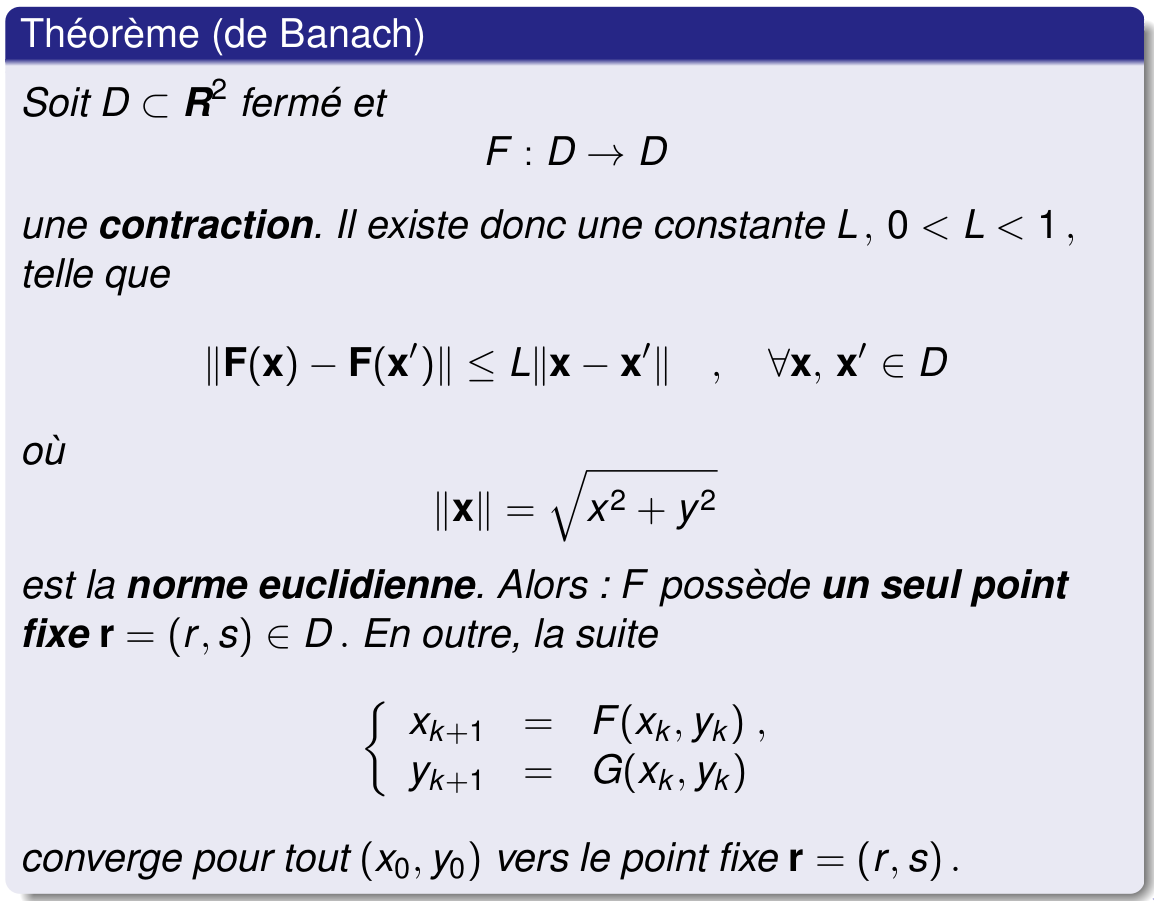
\includegraphics[width=0.45\textwidth]{img/banach_2.png}
    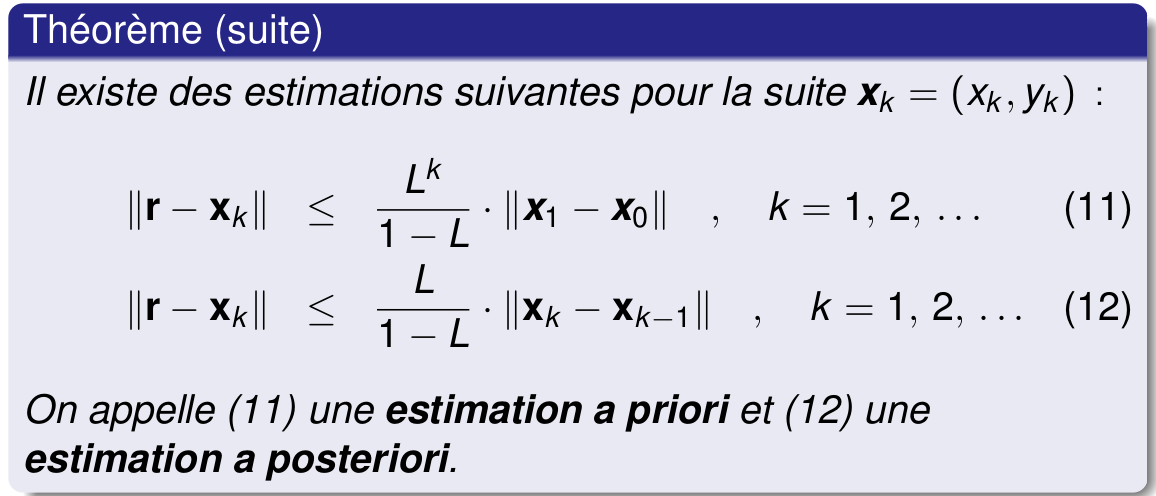
\includegraphics[width=0.45\textwidth]{img/banach_2_2.png}
\end{center}


\paragraph*{Exemple :}

Considérons la fonction $F$ suivante :
$$
F(x)= \matdd{F(x,y)}{G(x,y)} = \matdd{\frac{1}{10}(x^2+y^2+6)}{\frac{1}{10}(xy^2+x+5)}, \ \text{avec } x=\matdd{x}{y}
$$
La matrice de Jacobi est donnée par :
$$
J(x,y)=\matd{F_x(x,y)}{F_y(x,y)}{G_x(x,y)}{G_y(x,y)} = \frac{1}{10}\matd{2x}{2y}{y^2+1}{2xy}
$$
La norme matricielle est donnée par
$$
||J(x,y)||=\frac{1}{10}\sqrt{4x^2+4y^2+(y^2+1)^2+4x^2y^2}
$$
Si $\max_{(x,y)\in D}||J(x,y)||<1$ alors $F$ est une contraction.

Banach est un résultant théorique, en pratique c'est compliqué de trouvé un bon D.

Le vecteur d'erreur est donné par
$$
e_k = x_k - r = (\begin{array}{c}
x_k-r \\ 
y_k-s
\end{array} ) = (\begin{matrix}
\varepsilon_k \\ 
\delta_k
\end{matrix})
$$

Si $\textbf{J}(r,s)$ est nulle : convergence quadratique, sinon linéaire.

\section{Courbe de Bézier}
\subsection{L'algorithme de De Casteljau}
\subsubsection{Courbe de Bézier degré 2}
\begin{align*}
b_0^1(t) &= (1-t)b_0 + t\cdot b_1\\
b_1^1(t) &= (1-t)b_1 + t\cdot b_2\\
b_0^2(t) &= (1-t)b_0^1 + t\cdot b_1^1\\
b_0^2(t) &= (1-t)^2b_0 + 2t(1-t)\cdot b_1 + t^2b_2\\
\end{align*}
\begin{center}
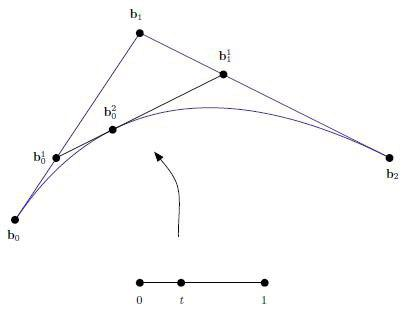
\includegraphics[width=0.4\textwidth]{img/bezier_1.jpg}\\ 
\end{center}
$$
b_0 = 
\begin{bmatrix}1\\1\end{bmatrix},
b_1 = 
\begin{bmatrix}2\\2.5\end{bmatrix},
b_2 = 
\begin{bmatrix}4\\1.5\end{bmatrix}
$$

\begin{align*}
& b_0^1(t) = (1-t)\begin{bmatrix}1\\1\end{bmatrix} + t\cdot \begin{bmatrix}2\\2.5\end{bmatrix}\\
& b_1^1(t) = (1-t)\begin{bmatrix}2\\2.5\end{bmatrix} + t\cdot \begin{bmatrix}4\\1.5\end{bmatrix}\\
& b_0^2(t) = (1-t)^2\begin{bmatrix}1\\1\end{bmatrix} + 2t(1-t)\cdot \begin{bmatrix}2\\2.5\end{bmatrix} + t^2\begin{bmatrix}4\\1.5\end{bmatrix}\\
& b_0^2(t) = 
\begin{bmatrix}
1+2t+t^2\\
1+3t+2.5t^2
\end{bmatrix}
\end{align*}

\paragraph*{Représentations des vecteurs:}
\begin{tabular}{lll}
$b_0$ &         &         \\
$b_1$ & $b_0^1$ &         \\
$b_2$ & $b_1^1$ & $b_0^2$
\end{tabular}
\subsubsection{Courbe de Bézier degré 3}

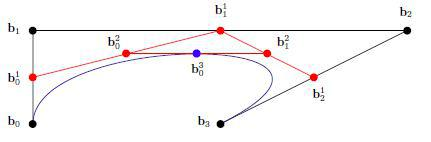
\includegraphics[width=0.4\textwidth]{img/bezier_2.jpg}

\paragraph*{Représentations des vecteurs:}
\begin{tabular}{llll}
$b_0$ &         &         & \\
$b_1$ & $b_0^1$ &         & \\
$b_2$ & $b_1^1$ & $b_0^2$ & \\
$b_3$ & $b_2^1$ & $b_1^2$ & $b_0^3$
\end{tabular}
\subsection{Polynôme de Bernstein}
$$B_i^n(t) = \begin{pmatrix}n\\i\end{pmatrix}t^i(1-t)^{n-i},(i=0,1,\cdots,n) $$

Facteur binonmiale:
$$\begin{pmatrix}n\\i\end{pmatrix} = \frac{n!}{i!\cdot(n-i)!}$$

\rotatebox{0}{
\begin{tiny}
\begin{tabular}{|l|l|l|l|l|}
\hline
$n$ & $i=0$              & $i=1$                & $i=2$                & $i=3$          \\ \hline\hline
0   & $B_0^0(t)=1$       &                      &                      &                \\ \hline
1   & $B_0^1(t)=1-t$     & $B_1^1(t)=t$         &                      &                \\ \hline
2   & $B_0^2(t)=(1-t)^2$ & $B_1^2(t)=2t(1-t)$   & $B_2^2(t)=t^2$       &                \\ \hline
3   & $B_0^3(t)=(1-t)^3$ & $B_1^3(t)=3t(1-t)^2$ & $B_2^3(t)=3t^2(1-t)$ & $B_3^3(t)=t^3$ \\ \hline
\end{tabular}
\end{tiny}
}
\subsection{Relation entre les courbes de Bézier et les polynômes de Bernstein}
$ b_0^1(t) = b_0B_0^1(t) + t\cdot b_1 $\\
$ b_1^1(t) = b_1B_0^1(t) + t\cdot b_2 $\\
$ b_0^2(t) = b_0B_0^2(t) + b_1B_1^2(t) + b_2B_2^2(t) $\\
$b_i^r(t) = \sum_{j=0}^r b_{i+j}B_j^r(t), 1\leq r \leq r, 0 \leq i \leq n-r$\\
Si $r=n$:\\$b_i^r(t) = \sum_{j=0}^n b_{j}B_j^n(t)$
\paragraph*{Tangente aux extrémité} $x'(t) = n \sum_{j=0}^{n-1}(b_{j+1-}-b_j)B_j^{n-1}(t)$
\subsection{Courbes de Bézier composées}
TODO:
\section{Méthode de Gauss}
\paragraph*{Exemple : }
$
A \vec{x} = \vec{b} \Longleftrightarrow
\begin{pmatrix}
 10 & -7 & 0       \\
 -3 & 2.059 &   6     \\
 5 &  -1 &   5     
\end{pmatrix}
\begin{pmatrix}
 x_1    \\
 x_2    \\
 x_3     
\end{pmatrix}
=
\begin{pmatrix}
 7  \\
 3.901    \\
 6     
\end{pmatrix}
\\
\Longleftrightarrow
\begin{pmatrix}[ccc|c]
 10 & -7 & 0   & 7    \\
 -3 & 2.059 &   6  & 3.901  \\
 5 &  -1 &   5 & 6  
\end{pmatrix}
$

\begin{tabular}{ll}
$l_{21} = \frac{a_{21}}{a_{11}} = - \frac{1}{3}$ & $l_{31} = \frac{a_{31}}{a_{11}} = - \frac{1}{2}$ \\
$L_2 - l_{21} \cdot L_1$ & $L_3 - l_{31} \cdot L_1$
\end{tabular}

\begin{tabular}{ll}
$
\begin{pmatrix}[ccc|c]
 10 & -7 & 0   & 7    \\
 0 & \fbox{-0.001} &   6  & 6.001  \\
 0 &  \fbox{2.5} &   5 & 2.5  
\end{pmatrix}
$
&
$
P=
\begin{pmatrix}
 1 & 0 & 0       \\
 0 & 1 & 0     \\
 0 & 0 & 1     
\end{pmatrix}
$
\end{tabular}

Le pivot de la ligne 3 est plus grand que celui de la ligne 2, les deux lignes dovent être intervertis.

\begin{tabular}{ll}
$
\begin{pmatrix}[ccc|c]
 10 & -7 & 0   & 7    \\
 0 &  \fbox{2.5} &   5 & 2.5  \\
 0 & \fbox{-0.001} &   6  & 6.001
\end{pmatrix}
$
&
$
P=
\begin{pmatrix}
 1 & 0 & 0       \\
 0 & 0 & 1     \\
 0 & 1 & 0     
\end{pmatrix}
$
\end{tabular}

\begin{tabular}{ll}
$l_{32} = \frac{a_{32}}{a_{22}} = -0.0004$ & $L_3 - l_{32} \cdot L_2$ 
\end{tabular}

\begin{tabular}{ll}
$
\begin{pmatrix}[ccc|c]
 10 & -7 & 0   & 7    \\
 0 &  2.5 &   5 & 2.5  \\
 0 & 0 &   6.002  & 6.002
\end{pmatrix}
$
&
$
U=
\begin{pmatrix}
 10 & -7 & 0      \\
 0 &  2.5 &   5   \\
 0 & 0 &   6.002  
\end{pmatrix}
$
\end{tabular}

\begin{tabular}{ll}
$
L=
\begin{pmatrix}
 1 & 0 & 0      \\
 l_{21} & 1 & 0   \\
 l_{31} & l_{32} & 1 
\end{pmatrix}
$
&
$
L=
\begin{pmatrix}
 1 & 0 & 0      \\
 -0.3333 & 1 & 0   \\
 0.5 & -0.0004 & 1 
\end{pmatrix}
$
\end{tabular}

Résoudre $L\cdot \vec{y} = \vec{b}$ et $U \cdot \vec{x} = \vec{y}$.

$
\begin{pmatrix}
 10 & -7 & 0      \\
 0 &  2.5 &   5   \\
 0 & 0 &   6.002  
\end{pmatrix}
\cdot \vec{x} =
\begin{pmatrix}
7\\
2.5\\
6.002
\end{pmatrix}
$

\section{Méthode A=QR}
\paragraph*{Buts : } Transformer une matrice A (quelconque) en une matrice triangulaire supérieur $R$. Où la norme des colonnes est préservée.
$
A = \begin{pmatrix}
\star & \star & \star & \star \\
\star & \star & \star & \star \\
\star & \star & \star & \star \\
\star & \star & \star & \star
\end{pmatrix}
\rightarrow \cdots \rightarrow
\begin{pmatrix}
\star & \star & \star & \star \\
0 & \star & \star & \star \\
0 & 0 & \star & \star \\
0 & 0 & 0 & \star
\end{pmatrix}
= R
$
\subsection{Matrice de Householder}
$
\rho = sign(x_1)||\vec{x}||_2, \quad \vec{v} = \vec{x} + \rho \vec{e_1},\quad \gamma = \frac{||\vec{v}||^2_2}{2} = \rho v_1
$

$
\vec{e_1} = 
\begin{pmatrix}
1\\
0\\
0\\
\vdots
\end{pmatrix}
$

Normalement nous n'aurons pas besoin de calculer la matrice de Householder

$
H = \begin{cases}
I, &\text{ si } v = 0 \\
I - \frac{vv^T}{\gamma} &\text{ si }v \neq 0
\end{cases}
$

\paragraph*{Exemple : } $x=(-2,2,1)^T$
\begin{align*}
&\rho = -\sqrt{(-2)^2 + (2)^2 + (1)^2} = -3 \\
& v = (-2,2,1) + (-3,0,0) = (-5,2,1) \\
& \gamma = \frac{(-5)^2+2^2+1^2}{2} = \frac{30}{2} = 15
\end{align*}
et on calcule $H$
\begin{align*}
H &= I - \frac{vv^T}{\gamma} = \frac{(-5,2,1) \cdot (-5,2,1)^T}{\gamma} \\
& = I - 
\frac{1}{15} \cdot \begin{pmatrix}
25 & -10 & -5 \\
-10 & 15 & 2 \\
-5 & 2 & 1
\end{pmatrix}\\
&=
\begin{pmatrix}
-\frac{2}{3} & \frac{2}{3} & \frac{1}{3} \\
\frac{2}{3} & \frac{11}{15} & -\frac{2}{15} \\
\frac{1}{3} & -\frac{2}{15} & \frac{14}{15}
\end{pmatrix}
\end{align*}

\paragraph*{Calcul de $H\vec{a}$ :}


$\tau = \frac{\vec{v}^T \vec{a}}{\gamma}$

$H\vec{a}=\vec{a}-\tau \vec{v}$

\paragraph*{Exemple:}

$a=(1,0,2)^T, \rho=-3, v=(-5,2,1)^T, \gamma = 15$ 

$\tau = -\frac{18}{15}, Ha = (-2,\frac{12}{5},\frac{16}{5})^T$

\paragraph*{Exemple de calcul de HA pour une matrice A}
$$
A = \begin{pmatrix}
2 & 4 & 2 \\
-1 & 0 & -4 \\
2 & 2 & -1
\end{pmatrix} = (\vec{a_1}|\vec{a_2}|\vec{a_3})
$$

\paragraph*{Exemple : } on reprend les algorithmes précédents et on calcule :
$$
\rho_1 = 3, v_1 = (5,-1,2)^T, \gamma_1 = 15
$$
puis on peut obtenir les éléments suivants :
$$
\tau_2 = \frac{v^T_1 a_2}{\gamma_1} = \frac{8}{5}, \quad 
\tau_3 = \frac{v^T_1 a_3}{\gamma_1} = \frac{4}{5}
$$
et donc
\begin{align*}
& H\vec{a_2} = \vec{a_2} - \tau_2\vec{v_1} = (-4,\frac{8}{5},-\frac{6}{5})^T \\
& H\vec{a_3} = \vec{a_3} - \tau_3\vec{v_1} = (-2,-\frac{16}{5},-\frac{13}{5})^T
\end{align*}

et obtient $HA$ :
$$
\begin{pmatrix}
-3 & -4 & -2 \\
0 & \frac{8}{5} & -\frac{16}{5} \\
0 & -\frac{6}{5} & -\frac{13}{5}
\end{pmatrix}
$$

\subsection{Méthode QR 1}
\paragraph*{Exemple : }
$$
A = \begin{pmatrix}
2 & 4 & 2 \\
-1 & 0 & -4 \\
2 & 2 & -1
\end{pmatrix} = (\vec{a_1}|\vec{a_2}|\vec{a_3})
$$

On a $H_1A$ suivante :
$$
H_1A = \begin{pmatrix}
-3 & -4 & -2 \\
0 & \frac{8}{5} & -\frac{16}{5} \\
0 & -\frac{6}{5} & -\frac{13}{5}
\end{pmatrix}
$$

et on travail sur $B$ :
$$
B = \begin{pmatrix}
\frac{8}{5} & -\frac{16}{5} \\
-\frac{6}{5} & -\frac{13}{5}
\end{pmatrix} = (\vec{b_2}|\vec{b_3})
$$

on cherche à obtenir $\overset{\sim}{H}_2B$ :
\begin{align*}
& \rho_2 = 2, \vec{v_2} = (\frac{18}{5},-\frac{6}{5})^T, \gamma_2=\frac{36}{5} \\
& \tau_4 = \frac{\vec{v_2}^T\vec{b_3}}{\gamma} = -\frac{7}{6}\\
& \overset{\sim}{H}_2\vec{b_3} = \vec{b_3} - \tau_4\vec{v_2} = (1,4)^T \\
& H_2 = 
\begin{pmatrix}[c|c]
1 & 0 \\ \hline
0 & \overset{\sim}{H}_2
\end{pmatrix}
\end{align*}

et on obtient :
$$
\begin{pmatrix}
-3 & -4 & -2 \\
0 & -2 & 1 \\
0 & 0 & -4
\end{pmatrix}
$$

\subsection{Résolution de $\textbf{Ax=b}$}

\paragraph*{si \textbf{A} est carré : } $A=QR$ et $Q^{-1}=Q^T$ donc $Ax=b \leftrightarrow QRx = b \leftrightarrow Rx = Q^Tb$
\paragraph*{si \textbf{A} est rectangulaire : } $A=QR$ et $Q^{-1}=Q^T$, $A^TAx=A^Tb$ donc $A^TAx=A^Tb\leftrightarrow Rx = Q^Tb$

Dans les deux cas, on ne construit pas $Q$. On applique l'algorithme de calcule de $HA$ pour une matrice $A$.

\section{Résolutions d'équations différentielles}

\subsection{Systèmes d'équations différentielles}
$y^{(n)} = f(t,y,y',\cdots,y^{(n-1)})$\\
$y_1=y,y_2=y',y_3=y'', \cdots y_n = y^{(n-1)}$\\
$
\begin{cases}
	y'_1 = y_2,\\
	y'_2 = y_3, \\
	\vdots\\
	y'_n=f(t,y_1,y_2,\cdots,y_n)
\end{cases}
$
\subsection{Méthode analytique}
\subsection{Méthode d'Euler}
$t_0=0$, $t_1=t_0+h$,...

$y'=\frac{dy}{dt}$

\begin{tabular}{ll}
$
\begin{cases}
y_{n+1} = y_n + hf(t_n,y_n), \\
t_{n+1} = t_n + h
\end{cases}
$
&
$n=0,1,2,\cdots$
\end{tabular}
\subsection{Erreur de troncature}
\subsection{Méthode à deux étages}
\subsubsection{Méthode du point milieu}
$
\begin{cases}
s_1 = f(t_n,y_n),\\
s_2 = f \left(t_n + \frac{h}{2}, y_n + \frac{1}{2}hs_1 \right),\\
y_{n+1} = y_n + hs_2, \\
t_{n+1} = t_n + h
\end{cases}
$
\subsubsection{Méthode du trapèze}

$
\begin{cases}
s_1 = f(t_n,y_n),\\
s_2 = f \left(t_n + h, y_n + hs_1 \right),\\
y_{n+1} = y_n + h\frac{s_1+s_2}{2}, \\
t_{n+1} = t_n + h
\end{cases}
$\\
Forme générale d'une méthode de Runge-Kutta:\\
$
\begin{cases}
s_1 = f(t_n,y_n),\\
s_2 = f \left(t_n + c_2h, y_n + a_{21}hs_1 \right),\\
y_{n+1} = y_n + h(\omega_1s_1+\omega_2s_2), \\
t_{n+1} = t_n + h
\end{cases}
$
\begin{tabular}{l|ll}
$0$   &            &            \\
$c_2$ & $a_{21}$     &            \\ \hline
      & $\omega_1$ & $\omega_2$
\end{tabular}\\
Pour la méthode du point milieu et du trapèze:\\
\begin{tabular}{l|ll}
$0$   &       &     \\
$1/2$ & $1/2$ &     \\ \hline
      & $0$   & $1$
\end{tabular}
\begin{tabular}{l|ll}
$0$ &       &       \\
$1$ & $1$   &       \\ \hline
    & $1/2$ & $1/2$
\end{tabular}\\
En prenant $c_2$ comme paramètre libre:\\
$\omega_1+\omega_2 = 1, \omega_2c_2=1/2,w_2a_{21}=1/2$
\begin{tabular}{l|ll}
$0$   &                    &                  \\
$c_2$ & $a_21$             &                  \\ \hline
      & $1-\frac{1}{2c_2}$ & $\frac{1}{2c_2}$
\end{tabular}
\subsection{Méthode à 3 étages}
$
\begin{cases}
s_1 = f(t_n,y_n),\\
s_2 = f \left(t_n + c_2h, y_n + a_{21}hs_1 \right),\\
s_3 = f \left(t_n + c_3h, y_n + a_{31}hs_1 + a_{32}hs_2 \right),\\
y_{n+1} = y_n + h(\omega_1s_1+\omega_2s_2 + \omega_3s_3), \\
t_{n+1} = t_n + h
\end{cases}
$

Tableau des paramètre:\\
\begin{tabular}{l|lll}
$0$   &            &            &            \\
$c_2$ & $a_{21}$   &            &            \\
$c_3$ & $a_{31}$   & $a_{32}$   &            \\ \hline
      & $\omega_1$ & $\omega_2$ & $\omega_3$
\end{tabular}

Exemples de tableau de différentes méthodes:\\
\begin{tabular}{l|lll}
$0$   &       &       &       \\
$1/2$ & $1/2$ &       &       \\
$1$   & $-1$  & $2$   &       \\ \hline
      & $1/6$ & $2/3$ & $1/6$
\end{tabular}
\begin{tabular}{l|lll}
$0$   &       &       &       \\
$1/2$ & $1/2$ &       &       \\
$3/4$ & $0$   & $3/4$ &       \\ \hline
      & $2/9$ & $3/9$ & $4/9$
\end{tabular}\\
\begin{tabular}{l|lll}
$0$   &       &       &       \\
$2/3$ & $2/3$ &       &       \\
$2/3$ & $1/3$ & $1/3$ &       \\ \hline
      & $1/4$ & $0$   & $3/4$
\end{tabular}

\subsection{Méthode de Runge-Kutta classique}
$
\begin{cases}
	s_1 = f(t_n,y_n),\\
	s_2 = f(t_n+1/2h,y_n+1/2hs_1),\\
	s_3 = f(t_n + 1/2h,y_n+1/2hs_2), \\
	s_4 = f(t_n + h,y_n+hs_3),\\
	y_{n+1} = y_n + h(1/6s_1 + 1/3s_2 + 1/3s_3 + 1/6s_4),\\
	t_{n+1} =t_n + h.
\end{cases}
$
\subsection{Méthode de Runge-Kutta Fehlberg}
$
\begin{cases}
	s_1 = f(t_n,y_n),\\
	s_2 = f(t_n+1/2h,y_n+1/2hs_1),\\
	s_3 = f(t_n + 3/4h,y_n+3/4hs_2), \\
	y_{n+1} = y_n + h/9(2s_1 + 3s_2 + 4s_3),
	s_4 = f(t_n + h,y_{n+1}),\\
	e_{n+1}=\frac{h}{72}(-5s_1+6s_2+8s_3-9s_4),\\
	t_{n+1} =t_n + h.
\end{cases}
$

\end{multicols*}
\end{document}

